
\chapter{Implementazione dei processi e delle primitive nel modulo sistema}

\section{Premessa: file \emph{include/costanti.h}}
Nel file \emph{sistema.s}, come in altri file di estensione cpp, è incluso con apposita direttiva il file \emph{costanti.h}
\begin{verbatim}
	#include "costanti.h"
\end{verbatim}
esso contiene una serie di costanti, tutte introdotte con \emph{define} per permetterne l'uso sia in C++ sia in Assembler. L'uso di queste costanti sarà evidente da qua fino alla fine della dispensa.

\section{Inizializzazione della \emph{Interrupt Descriptor Table}}
La gestione della \emph{Interrupt Descriptor Table} non è così diversa da quella vista con la libreria \emph{libce}.
\small 
\begin{verbatim}
	.global init_idt
	init_idt:
	//      indice      routine         dpl
	// gestori eccezioni:
	carica_gate	0       divide_error    LIV_SISTEMA
	carica_gate	1       debug           LIV_SISTEMA
	carica_gate	2       nmi             LIV_SISTEMA
	carica_gate	3       breakpoint      LIV_SISTEMA
	carica_gate	4       overflow        LIV_SISTEMA
	carica_gate	5       bound_re        LIV_SISTEMA
	carica_gate	6       invalid_opcode  LIV_SISTEMA
	carica_gate	7       dev_na          LIV_SISTEMA
	carica_gate	8       double_fault    LIV_SISTEMA
	carica_gate	9       coproc_so       LIV_SISTEMA
	carica_gate	10      invalid_tss     LIV_SISTEMA
	carica_gate	11      segm_fault      LIV_SISTEMA
	carica_gate	12      stack_fault     LIV_SISTEMA
	carica_gate	13      prot_fault      LIV_SISTEMA
	carica_gate	14      page_fault      LIV_SISTEMA
	// ... il tipo 15 è riservato
	carica_gate	16      fp_exc          LIV_SISTEMA
	carica_gate	17      ac_exc          LIV_SISTEMA
	carica_gate	18      mc_exc          LIV_SISTEMA
	carica_gate	19      simd_exc        LIV_SISTEMA
	carica_gate	20      virt_exc        LIV_SISTEMA
	// ... tipi 21-29 riservati
	carica_gate	30      sec_exc         LIV_SISTEMA
	// ... tipo 31 riservato
	
	// primitive comuni (tipi 0x2-)
	carica_gate	TIPO_A      a_activate_p    LIV_UTENTE
	carica_gate	TIPO_T      a_terminate_p   LIV_UTENTE
	carica_gate	TIPO_SI     a_sem_ini       LIV_UTENTE
	carica_gate	TIPO_W      a_sem_wait      LIV_UTENTE
	carica_gate	TIPO_S      a_sem_signal    LIV_UTENTE
	carica_gate	TIPO_D      a_delay         LIV_UTENTE
	carica_gate	TIPO_L      a_log           LIV_UTENTE
	carica_gate	TIPO_GMI    a_getmeminfo    LIV_UTENTE
	
	// primitive per il livello I/O (tipi 0x3-) 
	carica_gate	TIPO_APE    a_activate_pe   LIV_SISTEMA
	carica_gate	TIPO_WFI    a_wfi           LIV_SISTEMA
	carica_gate	TIPO_FG     a_fill_gate     LIV_SISTEMA
	carica_gate	TIPO_AB     a_abort_p       LIV_SISTEMA
	carica_gate	TIPO_IOP    a_io_panic      LIV_SISTEMA
	carica_gate	TIPO_TRA    a_trasforma     LIV_SISTEMA
	carica_gate	TIPO_ACC    a_access        LIV_SISTEMA
	
	// i tipi 0x4- verranno usati per le primitive fornite dal modulo I/O
	// (si veda fill_io_gates() in io.s)
	// i tipi da 0x50 a 0xFE verrano usati per gli handler
	// (si veda load_handler() più avanti)
	
	// la priorità massima è riservata al driver del timer di sistema
	carica_gate	TIPO_TIMER  driver_td       LIV_SISTEMA
	
	lidt idt_pointer
	ret
\end{verbatim}
\normalsize 
%\begin{center}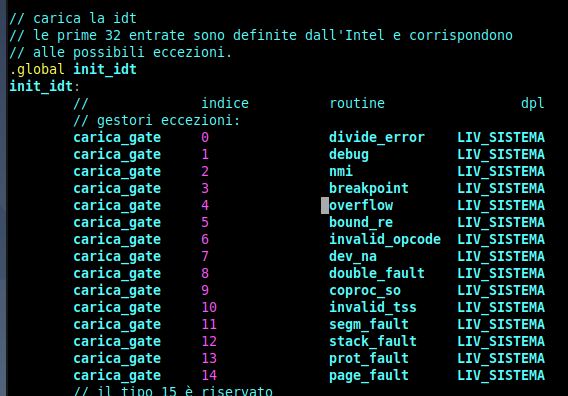
\includegraphics[scale=.75]{img/173.PNG}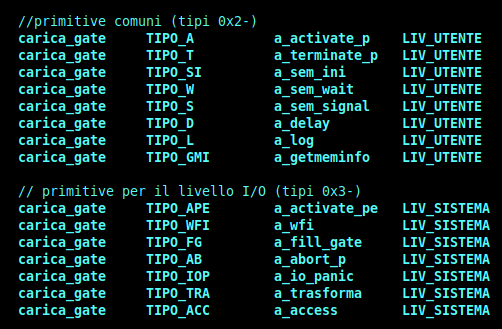
\includegraphics[scale=.75]{img/174.PNG}\end{center}
\begin{itemize}
	\item Abbiamo la \emph{carica$\_$gate}, ma con la possibilità di indicare anche il \emph{Descriptor Privilege Level} del gate (livello considerato solo nel lancio di interruzioni con istruzione INT). 
	\small
	\begin{verbatim}
		// Carica un gate della IDT
		// num: indice (a partire da 0) in IDT del gate da caricare
		// routine: indirizzo della routine da associare al gate
		// dpl: dpl del gate (LIV_SISTEMA o LIV_UTENTE)
		.macro carica_gate num routine dpl
		movq $\num, %rdi
		movq $\routine, %rsi
		movq $\dpl, %rdx
		xorq %rcx, %rcx
		call init_gate
		.endm
	\end{verbatim} 
	\normalsize
	\item \textbf{Attenzione}.
	
	Le righe di codice dove usiamo ripetutamente la macro \emph{carica$\_$gate} non sono il luogo dove effettivamente stiamo ponendo la nostra \emph{Interrupt Descriptor Table}. In fondo al file \emph{sistema.s} abbiamo uno spazio destinato a tale scopo
	\small
	\begin{verbatim}
		.bss
		.balign 16
		idt:
		// spazio per 256 gate
		// verra' riempita a tempo di esecuzione
		.space 16*256, 0
	\end{verbatim}
	\normalsize
	La routine \emph{init$\_$gate}, chiamata nella macro, organizza il contenuto di quell'area di memoria ogni volta che viene inserito un gate.
	
	\item \textbf{Istruzione LIDT}.
	
	Con l'istruzione \emph{lidt} andiamo ad aggiornare il registro IDTR 
	\begin{verbatim}
		lidt idt_pointer
	\end{verbatim}
	dove \emph{idt$\_$pointer} è una variabile avente una certa forma:
	\small
	\begin{verbatim}
		.data
		// ...
		idt_pointer:
		.word 0xFFF			// limite della IDT (256 entrate)
		.quad idt			// base della IDT
	\end{verbatim}
	\normalsize 
	\begin{itemize}
		\item il \emph{word} ci dicono quanto è grande la \emph{Interrupt Descriptor Table},
		\item il \emph{quad} contiene l'indirizzo della base della IDT (non a caso, \emph{idt}).
	\end{itemize}
	
	\item Ricordiamo quanto detto con l'APIC
	\small
	\begin{framed}
		\noindent Il livello di priorità è codificato nel tipo. L'identificativo può essere scomposto in due parti:
		\begin{itemize}
			\item la classe di priorità (parte più significativa), e 
			\item la sottopriorità all'interno della classe (parte meno significativa).
		\end{itemize}
		La regola che la APIC segue è di inviare una nuova richiesta di interruzione soltanto se tra quelle pendenti ce n'è una con classe di priorità maggiore della massima classe di priorità che è già stata accettata dal processore. In caso di \emph{ex-aequo} si guarda la sottopriorità.
	\end{framed}
	\normalsize Il primo parametro della \emph{carica$\_$gate} permette di indicare l'identificativo del tipo, dunque la priorità associata: maggiore è il valore numerico, maggiore sarà la priorità. Si osservi a chi viene attribuità la priorità massima: il timer (la cosa non dovrebbe stupirci)!
	\begin{verbatim}
		carica_gate TIPO_TIMER  driver_td       LIV_SISTEMA
	\end{verbatim}
	In \emph{include/costanti.h} sono definite una serie di costanti relative ai tipi dei gate
	\small
	\begin{multicols}{2}
		\begin{verbatim}
			// ( tipi delle primitive
			//   ( comuni
			#define TIPO_A			0x20	// activate_p
			#define TIPO_T			0x21	// terminate_p
			#define TIPO_SI			0x22	// sem_ini
			#define TIPO_W			0x23	// sem_wait
			#define TIPO_S			0x24	// sem_signal
			#define TIPO_D			0x25	// delay
			#define TIPO_L			0x26	// log
			#define TIPO_GMI		0x27	// getmeminfo (debug)
			//   )
			
			//   ( riservate per il modulo I/O
			#define TIPO_APE		0x30	// activate_pe
		\end{verbatim}
		\columnbreak 
		\begin{verbatim}
			#define TIPO_WFI		0x31	// wfi
			#define TIPO_FG			0x32	// fill_gate
			#define TIPO_AB			0x33	// abort_p
			#define TIPO_IOP		0x34	// io_panic
			#define TIPO_TRA		0x35	// trasforma
			#define TIPO_ACC		0x36	// access
			//   )
			
			// ...
			
			// tipo del driver del timer (priorità  massima)
			#define TIPO_TIMER		0xFF
		\end{verbatim}
	\end{multicols}
	\normalsize
	\item Possiamo classificare i gate già caricati in:
	\begin{itemize}
		\item eccezioni (dal gate 0 al gate 31, possibili eccezioni definite dalla Intel);
		\item primitive comuni (eseguibili a livello utente);
		\item primitive per il livello I/O (primitive che saranno utilizzate nel modulo I/O).
	\end{itemize}
	Altri gate saranno caricati più avanti, nel modulo I/O:
	\small 
	\begin{verbatim}
		// i tipi 0x4- verranno usati per le primitive fornite dal modulo I/O
		// (si veda fill_io_gates() in io.s)
		// i tipi da 0x50 a 0xFE verrano usati per gli handler
		// (si veda load_handler() più avanti)
	\end{verbatim}
	\normalsize 
	\item \textbf{Ma non è limitante usare un gate per ogni primitiva?} 
	
	Solitamente per tutte le primitive si usa un unico gate: la primitiva chiamata viene decisa sulla base di un valore posto in un registro (RAX, usa quel numero per accedere a un array di puntatori). In questo modo non siamo più limitati dall'hardware nel numero di primitive! Noi non faremo così: per quello che dobbiamo fare non ci serve un numero spropositato di primitive.
\end{itemize}

%\begin{center}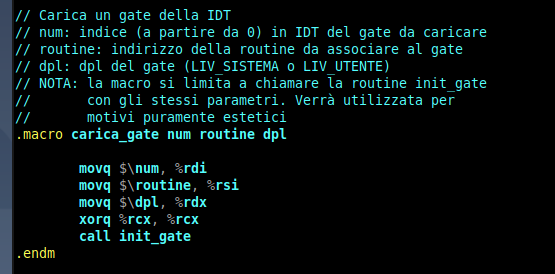
\includegraphics[scale=.8]{img/172.PNG}\end{center}

\section{Inizializzazione della \emph{Global Descriptor Table}}
Facciamo cose molto simili anche per la \emph{Global Descriptor Table}, che come già detto dobbiamo utilizzare (non come concepito all'inizio) per le modalità sistema e utente. All'interno della GDT troviamo anche il segmento TSS, che ci serve per gestire il cambio della pila.
\small 
\begin{verbatim}
	.balign 8
	.global gdt
	gdt:
	.quad 0		    //segmento nullo
	code_sys_seg:
	.word 0b0           //limit[15:0]   not used
	.word 0b0           //base[15:0]    not used
	.byte 0b0           //base[23:16]   not used
	.byte 0b10011010    //P|DPL|1|1|C|R|A|  DPL=00=sistema
	.byte 0b00100000    //G|D|L|-|-------|  L=1 long mode
	.byte 0b0           //base[31:24]   not used
	code_usr_seg:
	.word 0b0           //limit[15:0]   not used
	.word 0b0           //base[15:0]    not used
	.byte 0b0           //base[23:16]   not used
	.byte 0b11111010    //P|DPL|1|1|C|R|A|  DPL=11=utente
	.byte 0b00100000    //G|D|L|-|-------|  L=1 long mode
	.byte 0b0           //base[31:24]   not used
	data_usr_seg:
	.word 0b0           //limit[15:0]   not used
	.word 0b0           //base[15:0]    not used
	.byte 0b0           //base[23:16]   not used
	.byte 0b11110010    //P|DPL|1|0|E|W|A|  DPL=11=utente
	.byte 0b00000000    //G|D|-|-|-------|
	.byte 0b0           //base[31:24]   not used
	tss_seg:
	.space 16, 0	    // riempito da init_gdt
	end_gdt:
	
	tss:
	.long 0
	.global tss_punt_nucleo
	tss_punt_nucleo:
	.quad 0
	.space 11 * 8, 0
	.word 0
	.word tss_end - tss - 1
	tss_end:
\end{verbatim}
\normalsize 
Ci servono, come già anticipato:
\begin{itemize}
	\item un'entrata della GDT per gestire il passaggio da modalità utente a modalità sistema o per rimanere in modalità sistema;
	\item un'entrata della GDT per attraversare il gate e rimanere in modalità utente;
	\item il \emph{Task State Segment} per gestire il cambio della pila (nei modi già spiegati quando abbiamo affrontato l'implementazione della protezione nel processore Intel), di esso ci interessa solo la riga \emph{tss$\_$punt$\_$nucleo} (un \emph{quad} dove metteremo l'indirizzo della pila sistema ogni volta che cambiamo processo).
\end{itemize}
A un certo punto, da \emph{sistema.cpp}, verrà chiamata la funzione \emph{gdt$\_$init} (il cui codice si trova in \emph{sistema.s}). Non ci interessa il codice (Lettieri non l'ha neanche guardato), dobbiamo solo ricordarci che:
\begin{itemize}
	\item inizializza il contenuto del \emph{Task State Segment} (non è possibile farlo staticamente, nelle righe precedenti abbiamo solo preparato l'area di memoria);
	\item esegue la seguente istruzione
	\begin{verbatim}
		lgdt gdt_pointer
	\end{verbatim}
	dove \emph{gdt$\_$pointer} è un'area di ottanta byte con sintassi simile alla \emph{idt$\_$pointer}
	\begin{verbatim}
		.data
		gdt_pointer:
		.word end_gdt - gdt // limite della GDT
		.quad gdt
	\end{verbatim}
\end{itemize}
\small 
\normalsize 
%\begin{center}
\includegraphics[scale=.8]{img/177.PNG}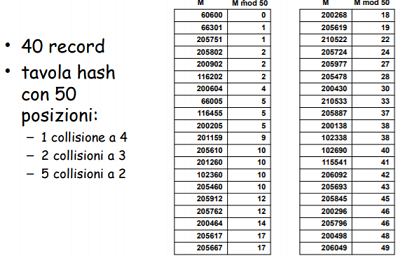
\includegraphics[scale=.8]{img/178.PNG}\end{center}



\section{Processo \emph{dummy} e shutdown con \emph{end$\_$program}}
Nella funzione \emph{main} di \emph{sistema.cpp} viene creato il cosiddetto \emph{processo dummy}.
\small 
\begin{verbatim}
	// creazione del processo dummy
	dummy_id = crea_dummy();
	if(dummy_id == 0xFFFFFFFF)
	goto error;
	flog(LOG_INFO, "Creato il processo dummy (id = %d)", dummy_id);
\end{verbatim}
\normalsize 
Esso permette di evitare il caso particolare in cui i processi sono tutti bloccati e non c'è altro da fare: risolvo la cosa con un processo a bassa priorità, dunque lo schedulatore trova sempre qualcosa da fare.
\subsection{Funzioni \emph{dummy} e \emph{crea$\_$dummy}}
\small
\begin{verbatim}
	extern "C" void end_program();
	void dummy(natq i) {
		while(processi)
		;
		end_program();
	}
	
	natl crea_dummy() {
		des_proc* di = crea_processo(dummy, 0, DUMMY_PRIORITY, LIV_SISTEMA, true);
		if(di == 0) {
			flog(LOG_ERR, "Impossibile creare il processo dummy");
			return 0xFFFFFFFF;
		}
		inserimento_lista(pronti, di);
		return di->id;
	}
\end{verbatim}
\normalsize 
%\begin{center}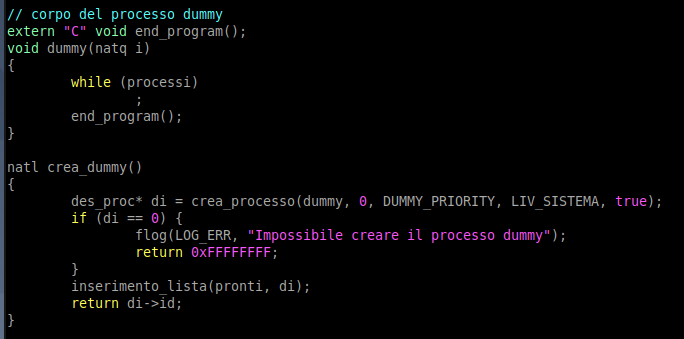
\includegraphics[scale=.9]{img/182.PNG}	
%	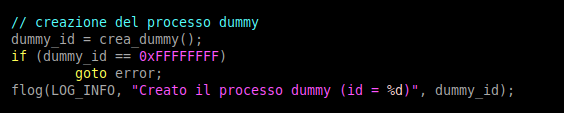
\includegraphics{img/181.PNG}\end{center}
La funzione \emph{dummy} si limita a guardare in continuazione la variabile \emph{processi}, che consiste nel numero di processi. Gira li finché il numero di processi attivi non sarà nullo\footnote{Ovviamente si tenga conto del passaggio a processi con priorità maggiore, cosa che avviene quando almeno un processo non è occupato.}.

\subsection{Funzione \emph{end$\_$program}} 
La funzione \emph{end$\_$program} verrà eseguita solo se non si hanno processi da eseguire, quindi se usciamo dal ciclo presente nella funzione \emph{dummy}. Il trucco consiste nel provocare un'eccezione di tipo \emph{abort}. Mette nella IDT un puntatore nullo (usando la LIDT) e lancia un'interruzione (con INT): nella IDT viene caricato un puntatore nullo, dunque trova l'indirizzo $0$ (non valido) e lancia un'eccezione di \emph{gate non valido}, anche in quel caso non trova l'indirizzo e lancia una terza eccezione che provoca \emph{abort} e quindi lo spegnimento.
\begin{verbatim}
	.global end_program
	end_program: 
	lidt triple_fault_idt 
	int $1
	
	// ...
	
	.data 
	triple_fault_idt:
	.word 0
\end{verbatim}
%\begin{center}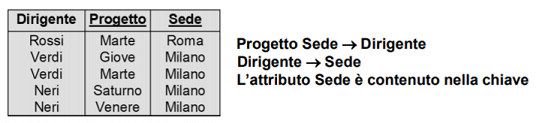
\includegraphics{img/183.PNG}\end{center}



\section{Strutture dati per la gestione dei processi}
\subsection{Descrittore di processo}
In \emph{sistema.cpp} abbiamo il descrittore di processo, già ampiamente descritto. 
\small 
\begin{verbatim}	
	const int N_REG = 16;
	struct des_proc {
		natw id;
		natw livello;
		natl precedenza;
		vaddr punt_nucleo; /* Puntatore a pila sistema */
		natq contesto[N_REG];
		paddr cr3;
		
		des_proc *puntatore;
	};
\end{verbatim}
\normalsize 
\subsection{Array dei processi}Tutti i descrittori di processo sono raccolti in un'array
\begin{verbatim}
	des_proc* proc_table[MAX_PROC];
\end{verbatim}
dove \emph{MAX$\_$PROC} è una costante posta in \emph{include/costanti.h}. 
\begin{verbatim}
	#define MAX_PROC        1024UL
\end{verbatim}
\subsection{Indici dei registri nell'array \emph{contesto}} Per quanto riguarda l'array \emph{contesto} si consideri l'\emph{enum} contenente i vari indici dei vari registri all'interno dell'array \emph{contesto}.
\begin{verbatim}
	enum { I_RAX, I_RCX, I_RDX, I_RBX, I_RSP, I_RBP, I_RSI, I_RDI, I_R8, I_R9, I_R10, 
		I_R11, I_R12, I_R13, I_R14, I_R15};
\end{verbatim}
quando andremo a manipolare i registri del contesto utilizzeremo queste costanti (non serve quindi conoscere l'indice preciso). \paragraph{Esempio}
\begin{verbatim}
	esecuzione->contesto[I_RAX] = true;
\end{verbatim}

\subsection{Puntatori}
Nel codice abbiamo questi due puntatori
\begin{verbatim}
	des_proc *esecuzione; 
	des_proc *pronti;
\end{verbatim}
\begin{itemize}
	\item \textbf{esecuzione} consiste nel puntatore all'unico processo in esecuzione nel processore.
	\item \textbf{pronti} è il puntatore alla testa di una lista di processi in attesa. La lista è costruita utilizzando, nella struttura \emph{des$\_$proc}, il puntatore \emph{puntatore}.
\end{itemize}

\subsection{Conteggio del numero di processi}
%Usando l'array precedente posso capire se un certo ID è già stato utilizzato: al momento della creazione di un processo scorro l'array finchè non ho un'entrata con \emph{null pointer}.
Poco dopo è definita la variabile \emph{processi}, che come già anticipato conteggia il numero di processi attivi.
\begin{verbatim}
	volatile natl processi;
\end{verbatim}
Viene posta \emph{volatile} poichè utilizzata nella funzione \emph{dummy}.

\section{Funzioni per la manipolazione delle liste}
In \emph{sistema.cpp} sono presenti delle funzioni che permettono di manipolare le liste. Ricordiamo che le liste relative ai processi sono ordinate esclusivamente in base alla precedenza. 
\subsection{Funzione \emph{inserimento$\_$lista}}
\small
\begin{verbatim}
	void inserimento_lista(des_proc* &p_lista, des_proc* p_elem) {
		// inserimento in una lista semplice ordinata
		// (tecnica dei due puntatori)
		des_proc *pp, *prevp;
		
		pp = p_lista;
		prevp = nullptr;
		while(pp && pp->precedenza >= p_elem->precedenza) {
			prevp = pp;
			pp = pp->puntatore;
		}
		
		p_elem->puntatore = pp;
		
		if(prevp)
		prevp->puntatore = p_elem;
		else
		p_lista = p_elem;
	}
\end{verbatim}
\normalsize 
\begin{itemize}
	\item La funzione \emph{inserimento$\_$lista} permette l'inserimento in una qualunque lista di un elemento \emph{des$\_$proc}. L'inserimento dell'elemento \emph{p$\_$elem} si basa sulle precedenze (chi ha precedenza più alta sta in cima alla lista), con logica FIFO (a parità di precedenza vince l'elemento inserito per primo nella lista).
	\item Il parametro di ingresso \emph{p$\_$lista} è il puntatore alla lista da manipolare (con riferimento, potrei porre un elemento in cima alla lista). 
	\item Il parametro di ingresso \emph{p$\_$elem} è il puntatore all'elemento da inserire nella lista.
	\item Il codice è simile, se non identico, alla funzione studiata a \emph{Fondamenti di programmazione} per l'inserimento di un elemento in una lista: 
	\begin{itemize}
		\item scorro la lista finché non trovo il punto dove il processo deve essere inserito;
		\item modifico \emph{puntatore} dell'elemento precedente e imposto \emph{puntatore} del processo appena inserito.
	\end{itemize}
\end{itemize}
\subsection{Funzione \emph{rimozione$\_$lista}}
\small
\begin{verbatim}
	des_proc* rimozione_lista(des_proc* &p_lista) {
		// estrazione della testa
		des_proc *p_elem = p_lista // nullptr se la lista e' vuota
		
		if(p_lista)
		p_lista = p_lista->puntatore;
		
		if(p_elem)
		p_elem->puntatore = nullptr;
		
		return p_elem;
	}
\end{verbatim}
\normalsize
\begin{itemize}
	\item La funzione \emph{rimozione$\_$lista} permette la rimozione della testa di una qualunque lista di elementi \emph{des$\_$proc}.
	\item Il parametro di ingresso \emph{p$\_$lista} è il puntatore alla lista (con riferimento, visto che rimuoviamo la testa).
	\item Pongo nel puntatore \emph{p$\_$elem} l'indirizzo della testa.
	\item Se nella lista puntata da \emph{p$\_$lista} sono presenti elementi (prima di procedere all'estrazione) modifico il puntatore \emph{p$\_$lista} rendendo il secondo elemento la nuova testa.
	\item Se l'elemento estratto non è nullo modifico il suo \emph{puntatore} ponendolo a null (lo abbiamo scollegato dalla lista, non ha senso mantenere un collegamento).
	\item Restituisco l'indirizzo della testa estratta (\emph{p$\_$elem}).
\end{itemize}

\subsection{Funzione \emph{inspronti} per la lista \emph{pronti}}
\small
\begin{verbatim}
	extern "C" void inspronti() {
		esecuzione->puntatore = pronti;
		pronti = esecuzione;
	}
\end{verbatim}
\normalsize 
La funzione \emph{inspronti} inserisce il processo attualmente in esecuzione in testa alla lista \emph{pronti}. Si consideri che:
\begin{itemize}
	\item se abbiamo lavorato bene inseriremo in testa il processo con priorità maggiore;
	\item abbiamo aggiornato la lista \emph{pronti}, \textbf{ma non abbiamo modificato \emph{esecuzione}} (il processo posto in \emph{esecuzione} è sempre quello attualmente in esecuzione).
\end{itemize}

\subsection{Funzione \emph{schedulatore} per la lista \emph{pronti}}
\[\boxed{\text{\textbf{Promemoria}. La schedulazione è il passaggio di un processo da \emph{pronto} a \emph{esecuzione}}}\]
La funzione \emph{schedulatore} comporterà il passaggio di un processo (quello con priorità maggiore) dallo stato \emph{pronto} a \emph{esecuzione}. Le cose da fare sono due:
\begin{enumerate}
	\item estrarre la testa dalla coda \emph{pronti} (in testa abbiamo, secondo logica FIFO, il processo con priorità maggiore);
	\item fare puntare il processo appena estratto dal puntatore \emph{esecuzione}.
\end{enumerate}
Grazie alla funzione \emph{rimozione$\_$lista} il codice della funzione \emph{schedulatore} è molto breve.
\small
\begin{verbatim}
	extern "C" void schedulatore(void) {
		esecuzione = rimozione_lista(pronti);
	}
\end{verbatim}
\normalsize
\paragraph{Attenzione} La funzione sceglie soltanto il processo che dovrà andare in esecuzione quando è finita la primitiva! \textbf{Non si ha il cambio di processo nel momento in cui chiamiamo schedulatore}. \textit{Se pensate che scrivere dentro una variabile basti per cambiare il processo allora avete le idee un po' confuse (cit.)}.

\section{Funzioni \emph{salva$\_$stato} e \emph{carica$\_$stato}}

Nel file \emph{sistema.s} abbiamo due funzioni familiari: \emph{salva$\_$stato} e \emph{carica$\_$stato}. Nulla di strano, solo un qualcosa di intricato.

\subsection{Premessa: offset}
Sono definite in Assembler una serie di costanti per gestire gli offset:
\small 
\begin{verbatim}
	// offset dei vari registri all'interno di des_proc
	.set PUNT_NUCLEO, 8
	.set CTX, 16
	.set RAX, CTX+0
	.set RCX, CTX+8
	.set RDX, CTX+16
	.set RBX, CTX+24
	.set RSP, CTX+32
	.set RBP, CTX+40
	.set RSI, CTX+48
	.set RDI, CTX+56
	.set R8,  CTX+64
	.set R9,  CTX+72
	.set R10, CTX+80
	.set R11, CTX+88
	.set R12, CTX+96
	.set R13, CTX+104
	.set R14, CTX+112
	.set R15, CTX+120
	.set CR3, CTX+128
\end{verbatim}
\normalsize 
In entrambe le funzioni gli offset vengono utilizzati rispetto al registro RBX, dove abbiamo posto \emph{esecuzione} (quindi gli offset sono costruiti tenendo conto della struttura di \emph{des$\_$proc})
\begin{verbatim}
	movq esecuzione, %rbx
\end{verbatim}
\subsection{salva$\_$stato}	
\small 
\begin{verbatim}
	// copia lo stato dei registri generali nel des_proc del processo puntato da
	// esecuzione.  Nessun registro viene sporcato.
	
	salva_stato:
	// salviamo lo stato di un paio di registri in modo da poterli
	// temporaneamente riutilizzare. In particolare, useremo %rax come
	// registro di lavoro e %rbx come puntatore al des_proc.
	pushq %rbx
	pushq %rax
	
	movq esecuzione, %rbx
	
	// copiamo per primo il vecchio valore di %rax
	movq (%rsp), %rax
	movq %rax, RAX(%rbx)
	// usiamo %rax come appoggio per copiare il vecchio %rbx
	movq 8(%rsp), %rax
	movq %rax, RBX(%rbx)
	// copiamo gli altri registri
	movq %rcx, RCX(%rbx)
	movq %rdx, RDX(%rbx)
	// salviamo il valore che %rsp aveva prima della chiamata a salva stato
	// (valore corrente meno gli 8 byte che contengono l'indirizzo di
	// ritorno e i 16 byte dovuti alle due push che abbiamo fatto all'inizio)
	movq %rsp, %rax
	addq $24, %rax
	movq %rax, RSP(%rbx)
	movq %rbp, RBP(%rbx)
	movq %rsi, RSI(%rbx)
	movq %rdi, RDI(%rbx)
	movq %r8,  R8 (%rbx)
	movq %r9,  R9 (%rbx)
	movq %r10, R10(%rbx)
	movq %r11, R11(%rbx)
	movq %r12, R12(%rbx)
	movq %r13, R13(%rbx)
	movq %r14, R14(%rbx)
	movq %r15, R15(%rbx)
	
	popq %rax
	popq %rbx
	
	ret
\end{verbatim}
\normalsize 
\begin{itemize}
	\item La funzione deve essere chiamata subito dopo essere entrati nel modulo sistema, per qualunque motivo. Deve memorizzare lo stato di tutti i registri nel momento in cui è stata chiamata. 
	\item I registri che utilizziamo per svolgere le nostre operazioni sono RAX ed RBX. Il primo è utilizzato come registro di lavoro (cioè per fare passi intermedi), mentre RBX lo usiamo per puntare al descrittore di processo corrente (posto nella variabile globale \emph{esecuzione}). Per fare queste cose poniamo in pila il contenuto vecchio di RAX ed RBX
	\begin{verbatim}
		pushq %rbx
		pushq %rax
	\end{verbatim}
	%\begin{center}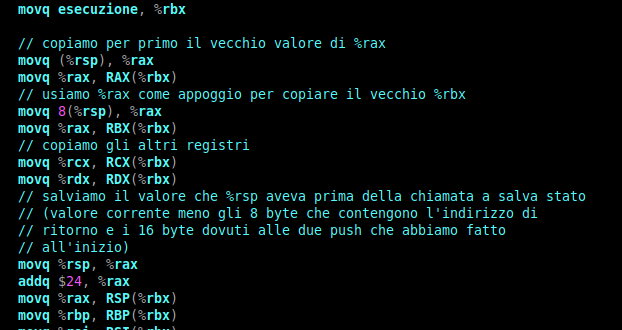
\includegraphics[scale=.9]{img/184.PNG}\end{center}
	\item Pongo in rbx il contenuto della variabile globale \emph{esecuzione} 
	\begin{verbatim}
		movq esecuzione, %rbx
	\end{verbatim}
	\item Pongo nel \emph{contesto} il contenuto di RAX
	\item Pongo nel \emph{contesto} il contenuto di RBX, utilizzando RAX come registro di lavoro (ho bisogno di un registro dove spostare il mio risultato intermedio, per forza).
	\item Segue una sfilata di costanti attraverso cui indichiamo i relativi offset e spostiamo in \emph{contesto} il contenuto dei registri rimanenti.
	\item Per porre il valore vecchio di RSP dobbiamo ricordarci che abbiamo eseguito una chiamata di funzione e due push, dunque RSP è già stato spostato rispetto all'inizio. Segue
	\begin{verbatim}
		movq %rsp, %rax
		addq $24, %rax
	\end{verbatim} Useremo il valore vecchio calcolato nella IRETQ per la lettura della pila sistema.
	\item Esegiamo le due pop consuete dopo aver finito di utilizzare i registri RAX ed RBX
	\begin{verbatim}
		pop %rax
		pop %rbx
	\end{verbatim}
\end{itemize}

\subsection{carica$\_$stato}
\small 
\begin{verbatim}
	// carica nei registri del processore lo stato contenuto nel des_proc del
	// processo puntato da esecuzione.  Questa funzione sporca tutti i registri.
	carica_stato:
	movq esecuzione, %rbx
	
	popq %rcx   //ind di ritorno, va messo nella nuova pila
	
	// nuovo valore per cr3
	movq CR3(%rbx), %r10
	movq %cr3, %rax
	cmpq %rax, %r10
	je 1f			// evitiamo di invalidare il TLB
	// se cr3 non cambia
	movq %r10, %rax
	movq %rax, %cr3		// il TLB viene invalidato
	1:
	// anche se abbiamo cambiato cr3 siamo sicuri che l'esecuzione prosegue
	// da qui, perché ci troviamo dentro la finestra FM che è comune a
	// tutti i processi
	movq RSP(%rbx), %rsp    //cambiamo pila
	pushq %rcx              //rimettiamo l'indirizzo di ritorno
	
	// se il processo precedente era terminato o abortito la sua pila
	// sistema non era stata distrutta, in modo da permettere a noi di
	// continuare ad usarla. Ora che abbiamo cambiato pila possiamo
	// disfarci della precedente.
	cmpq $0, ultimo_terminato
	je 1f
	call distruggi_pila_precedente
	1:
	// aggiorniamo il puntatore alla pila sistema usata dal meccanismo
	// delle interruzioni
	movq PUNT_NUCLEO(%rbx), %rcx
	movq %rcx, tss_punt_nucleo
	
	movq RCX(%rbx), %rcx
	movq RDI(%rbx), %rdi
	movq RSI(%rbx), %rsi
	movq RBP(%rbx), %rbp
	movq RDX(%rbx), %rdx
	movq RAX(%rbx), %rax
	movq R8(%rbx), %r8
	movq R9(%rbx), %r9
	movq R10(%rbx), %r10
	movq R11(%rbx), %r11
	movq R12(%rbx), %r12
	movq R13(%rbx), %r13
	movq R14(%rbx), %r14
	movq R15(%rbx), %r15
	movq RBX(%rbx), %rbx
	
	retq
\end{verbatim}
\normalsize 
%\begin{center}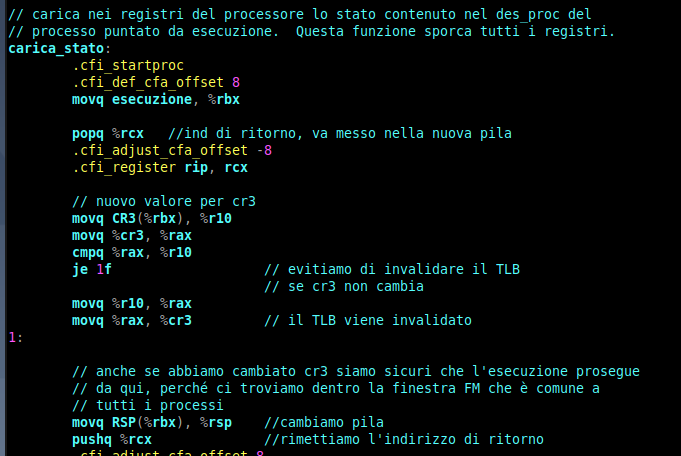
\includegraphics[scale=.9]{img/185.PNG}\end{center}
\begin{itemize}
	\item La funzione ha un problema: è stata chiamata, il suo indirizzo di ritorno è stato messo nella pila corrente, se il valore di \emph{esecuzione} è stato modificato a un certo punto tra tutti i registri caricherà anche rsp. La pila punterà da un'altra parte, ma l'indirizzo di ritorno si trova nella vecchia pila. Dobbiamo complicarci un attimo la vita per spostare l'indirizzo di ritorno dalla pila vecchia a quella nuova.
	\item Verifico se il processo precedente è stato terminato o abortito. In quel caso la pila sistema può essere distrutta (se terminiamo un processo allora la pila sistema relativa al processo non sarà più utilizzata).
	\item Pongo in RBX, come prima, l'indirizzo al descrittore di processo
	\begin{verbatim}
		movq esecuzione, %rbx
	\end{verbatim}
	\item Metto in RCX l'indirizzo di ritorno, lo levo dalla pila precedente.
	\item Il registro CR3 viene affrontato nel capitolo sulla paginazione.
	\item Modifico RSP mettendo il valore relativo alla nuova pila.
	\item Eseguo la POP per inserire nella nuova pila l'indirizzo di ritorno
	\begin{verbatim}
		pushq %rcx
	\end{verbatim}
	\item A questo punto carico tutti i registri. 
	\item In più, aggiorno \emph{tss$\_$punt$\_$nucleo}  nel TSS (ricordare quanto deciso sull'uso del TSS - univoco per tutti i processi, con necessità di modificare ogni volta il puntatore alla pila sistema nel TSS stesso).
	%\begin{center}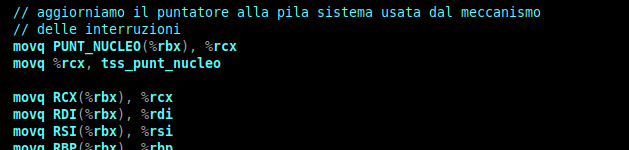
\includegraphics[scale=.9]{img/186.PNG}\end{center}
\end{itemize}




\section{Primitive}
Il codice di una primitiva è sempre strutturato in due parti:
\begin{itemize}
	\item una parte in Assembler dove eseguiamo all'inizio la \emph{salva$\_$stato} e alla fine la \emph{carica$\_$stato};
	\item una routine scritta in C++, chiamata tra le due funzioni appena citate.
\end{itemize}
Il codice vero e proprio della primitiva è posto nella routine.
\subsection{Funzione di utilità \emph{liv$\_$chiamante}}
\[\boxed{\text{Funziona solo se è stata chiamata la \emph{salva$\_$stato}}}\]
La funzione \emph{liv$\_$chiamante} restituisce il livello di privilegio a cui si trovava il processore nel momento in cui è stata invocata la primitiva.
\small 
\begin{verbatim}
	int liv_chiamante() {
		// salva_stato ha salvato il puntatore alla pila sistema
		// subito dopo l'invocazione della INT
		natq *pila = reinterpret_cast<natq*>(esecuzione->contesto[I_RSP]);
		
		// la seconda parola dalla cima della pila contiene il livello
		// di privilegio che aveva il processore prima della INT
		return pila[1] == SEL_CODICE_SISTEMA ? LIV_SISTEMA : LIV_UTENTE;
	}
\end{verbatim}
\normalsize
\begin{itemize}
	\item La funzione recupera dal registro RSP nel contesto la pila.
	\item Dalla seconda \emph{quadword} nella pila (indice $1$) viene recuperato il \emph{Current Privilege Level}.
	\item Abbiamo utilizzato alcune costanti poste in \emph{include/costanti.h}
	\begin{verbatim}
		#define SEL_CODICE_SISTEMA        0x8
		#define LIV_UTENTE        3
		#define LIV_SISTEMA        0
	\end{verbatim}
\end{itemize}
\paragraph{Perchè non usare \emph{punt$\_$nucleo}?} L'indirizzo in \emph{punt$\_$nucleo} è quello della base della pila. Noi non sappiamo quale sia la distanza tra la base e la \emph{quadword} che ci interessa.
\subsection{Analisi della struttura della primitiva \emph{activate$\_$p}}
\subsubsection{Parte Assembler}
\small 
\begin{verbatim}
	.extern c_activate_p
	a_activate_p:
	call salva_stato
	call c_activate_p
	call carica_stato
	iretq
\end{verbatim}
\normalsize 
Abbiamo il solito incapsulamento con \emph{salva$\_$stato} (eseguita prima della parte C++ della primitiva) e \emph{carica$\_$stato} (eseguita dopo la parte C++ della primitiva). Nulla di particolare rispetto a quanto già detto.
\subsubsection{Parte C++}
\small 
\begin{verbatim}
	extern "C" void c_activate_p(void f(natq), natq a, natl prio, natl liv) {
		des_proc *p;			// des_proc per il nuovo processo
		natl id = 0xFFFFFFFF;		// id da restituire in caso di fallimento
		
		// non possiamo accettare una priorita'  minore di quella di dummy
		// o maggiore di quella del processo chiamante
		if (prio < MIN_PRIORITY || prio > esecuzione->precedenza) {
			flog(LOG_WARN, "priorita' non valida: %d", prio);
			c_abort_p();
			return;
		}
		
		// controlliamo che 'liv' contenga un valore ammesso
		// [segnalazione di E. D'Urso]
		if (liv != LIV_UTENTE && liv != LIV_SISTEMA) {
			flog(LOG_WARN, "livello non valido: %d", liv);
			c_abort_p();
			return;
		}
		
		// non possiamo creare un processo di livello sistema mentre
		// siamo a livello utente
		if (liv == LIV_SISTEMA && liv_chiamante() == LIV_UTENTE) {
			flog(LOG_WARN, "errore di protezione");
			c_abort_p();
			return;
		}
		
		// accorpiamo le parti comuni tra c_activate_p e c_activate_pe
		// nella funzione ausiliare crea_processo
		p = crea_processo(f, a, prio, liv, (liv == LIV_UTENTE));
		
		if (p != nullptr) {
			inserimento_lista(pronti, p);
			processi++;
			id = p->id;			// id del processo creato
			// (allocato da crea_processo)
			flog(LOG_INFO, "proc=%d entry=%p(%d) prio=%d liv=%d", id, f, a, prio, liv);
		}
		
		esecuzione->contesto[I_RAX] = id;
	}
\end{verbatim}
\normalsize 
\begin{itemize}
	\item La \emph{c$\_$activate$\_$p} è l'implementazione vera e propria della primitiva \emph{activate$\_$p}, scritta in C++. 
	\begin{itemize}
		\item Si osservi il primo parametro di ingresso
		\begin{verbatim}
			void f(natq)
		\end{verbatim}
		esso è un puntatore a funzione, una funzione avente come unico parametro in ingresso \emph{natq}. Porremo questo valore attraverso il secondo parametro di ingresso.
		\item Vengono posti una serie di controlli per verificare la validità dei parametri in ingresso
		\begin{itemize}
			\item Verifico se la priorità posta dall'utente col parametro \emph{prio} sia minore della priorità minima e/o maggiore della priorità del processo attualmente in esecuzione. La prima cosa deve essere evitata, visto che non posso avere processi con priorità più bassa di \emph{dummy}, la seconda è una forma di semplificazione.
			\item Verifico se il livello posto con \emph{liv} sia un valore valido.
			\item Verifico che non venga richiesta l'attivazione di un processo a livello sistema da parte di un chiamante a livello utente (abbiamo già detto che possiamo creare processi di questo livello solo a livello sistema). Il livello del chiamante viene ottenuto con la funzione di utilità \emph{liv$\_$chiamante}.
		\end{itemize}
	\end{itemize}
	\item Alla fine creo effettivamente il processo con un'altra funzione, che possiamo ignorare (cit.)
	\begin{verbatim}
		p = crea_processo(f, a, prio, liv, (liv == LIV_UTENTE));
	\end{verbatim}
	Se tutto va bene la funzione mi restituisce l'ID univoco del processo creato.
	\item Incremento \emph{processo}, variabile globale che conteggia il numero di processi esistenti. Stampo un avviso con i dati di base relativi al processo.
	\begin{framed}
		\item La primitiva deve restituire al chiamante l'id del processo chiamato. Questo è stato allocato dalla \emph{crea$\_$processo}, che lo ha posto nel descrittore di processo. Per restituirlo stiamo facendo in modo diverso da una \emph{return}
		\begin{verbatim}
			esecuzione->contesto[I_RAX] = id;
		\end{verbatim}
		\textbf{Come mai?} 
		
		Perchè la \emph{carica$\_$stato} sovrascrive quanto posto se poniamo direttamente il valore in RAX. Il valore di \emph{esecuzione}, non è stato modificato, dunque indica il processo che ha invocato l'\emph{activate$\_$p}. Ricordarsi la funzione del registro RAX nella traduzione C++-Assembler.
	\end{framed}
\end{itemize}

\subsubsection{Invocazione della primitiva da parte di un utente}
Poniamoci un'ulteriore domanda...
\paragraph{Come fa l'utente a chiamare la primitiva?} Noi abbiamo parlato solo di funzioni che hanno prefisso \emph{a} (Assembler) o \emph{c} (C++), ma l'utente chiama cose senza prefissi. Sappiamo che dobbiamo eseguire un'istruzione INT. Noi nel codice poniamo una cosa del genere
\begin{verbatim}
	activate_p(f, 10, 10, LIV_UTENTE);
\end{verbatim}
dal punto di vista del C++ stiamo chiamando una normale funzione C++. Vediamo il codice che si cela dietro
\small 
\begin{verbatim}
	.global activate_p
	activate_p:
	int $TIPO_A
	ret
\end{verbatim}
\normalsize 
%\begin{center}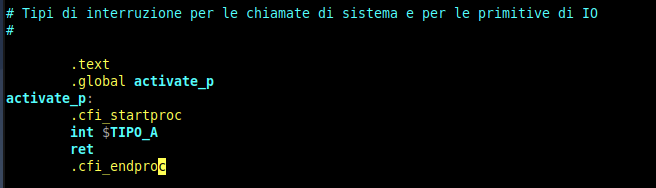
\includegraphics[scale=.76]{img/190.PNG}\end{center}
Abbiamo una \textbf{funzione di appoggio} scritta in Assembler (per forza, non posso eseguire la INT in C++). L'identificativo del tipo dell'interruzione relativa alla primitiva deve essere noto: poniamo per comodità le costanti \emph{TIPO$\_$x} nel file \emph{include/costanti.h}.

\paragraph{Effetto dell'esecuzione di INT?} Lancio di \emph{a$\_$activate$\_$p}. I parametri posti in ingresso non sono stati modificati e possono essere usati.

\subsection{Esempio di primitiva creata da noi: \emph{getprec}}
Proviamo a creare una nostra primitiva, cosa che tipicamente si fa negli esercizi di esame.
\paragraph{Cosa dobbiamo fare?} Facciamo una primitiva con cui un processo può farsi dire dal sistema qual è la sua precedenza.
\begin{itemize}
	\item \textbf{Assegnazione di un identificativo al tipo di interruzione}. 
	
	La prima cosa da fare è assegnare un numero. Vado in \emph{costanti.h} e definisco una nuova costante con la direttiva define
	\begin{verbatim}
		#define TIPO_GETPREC     0x28
	\end{verbatim}
	Ovviamente poniamo un numero che non è ancora utilizzato.
	
	\item \textbf{Aggiungo un gate nell'IDT}.
	
	Modifico il codice relativo al caricamento dell'IDT in \emph{sistema.s}. Carico un gate 
	\begin{verbatim}
		carica_gate     TIPO_GETPREC     a_getprec     LIV_UTENTE
	\end{verbatim}
	chiaramente devo mettere \emph{LIV$\_$UTENTE}, altrimenti non potremo chiamare la primitiva.
	
	\item \textbf{Funzione di "incapsulamento" con \emph{salva} e \emph{carica} stato}. 
	
	In \emph{utenti.s} scriviamo \emph{a$\_$getprec}. La struttura è sempre la stessa
	\begin{verbatim}
		a_getprec:
		call salva_stato
		call c_getprec
		call carica_stato
		iretq
	\end{verbatim}
	
	\item \textbf{Implementazione concreta della primitiva}. 
	
	Scriviamo il succo della primitiva in C++ (cioè scriviamo la funzione \emph{c$\_$getprec} chiamata tra la \emph{salva$\_$stato} e la \emph{carica$\_$stato}).
	\begin{verbatim}
		extern "C" void c_getprec() {
			esecuzione->contesto[I_RAX] = esecuzione->precedenza;
		}
	\end{verbatim}
	Chiaramente una cosa del genere può essere fatta solo in modalità sistema, unico modo per accedere ad \emph{esecuzione} e a ciò che punta \emph{esecuzione} stesso.
	\item \textbf{Funzione di appoggio}. 
	
	No, l'utente non può ancora chiamare la primitiva in C++: manca la funzione di appoggio che esegue la INT. Andiamo in \emph{include/sys.h}, dove dichiariamo la nostra primitiva
	\begin{verbatim}
		extern "C" natl getprec();
	\end{verbatim}
	Poi, in \emph{utente/utente.s}, scriviamo quanto segue
	\begin{verbatim}
		getprec:    
		int $TIPO_GETPREC
		ret
	\end{verbatim}
	Adesso abbiamo davvero finito.
\end{itemize}
\paragraph{Esempio di chiamata della primitiva}
\begin{verbatim}
	#include <all.h>
	void f(natq a) {
		prinft("La mia precedenza e' %d\n", getprec());
		terminate_p();
	}
	
	void main() {
		activate_p(f, 10, 10, LIV_UTENTE);
		terminate_p();
	}
\end{verbatim}
L'output restituisce la precedenza indicata nell'apposito parametro di ingresso di \emph{activate$\_$p}.
\begin{center}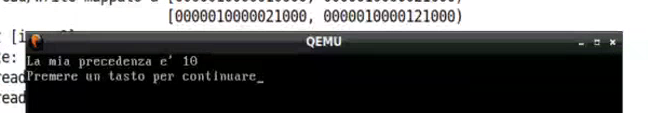
\includegraphics[scale=.95]{img/191.PNG}\end{center}